\documentclass[12pt]{article}

\usepackage{../thesis}

\usepackage{tikz} 

\begin{document}

\pagestyle{empty}

\begin{tikzpicture}
    \node[anchor=south west,inner sep=0] (image) at (0,0) {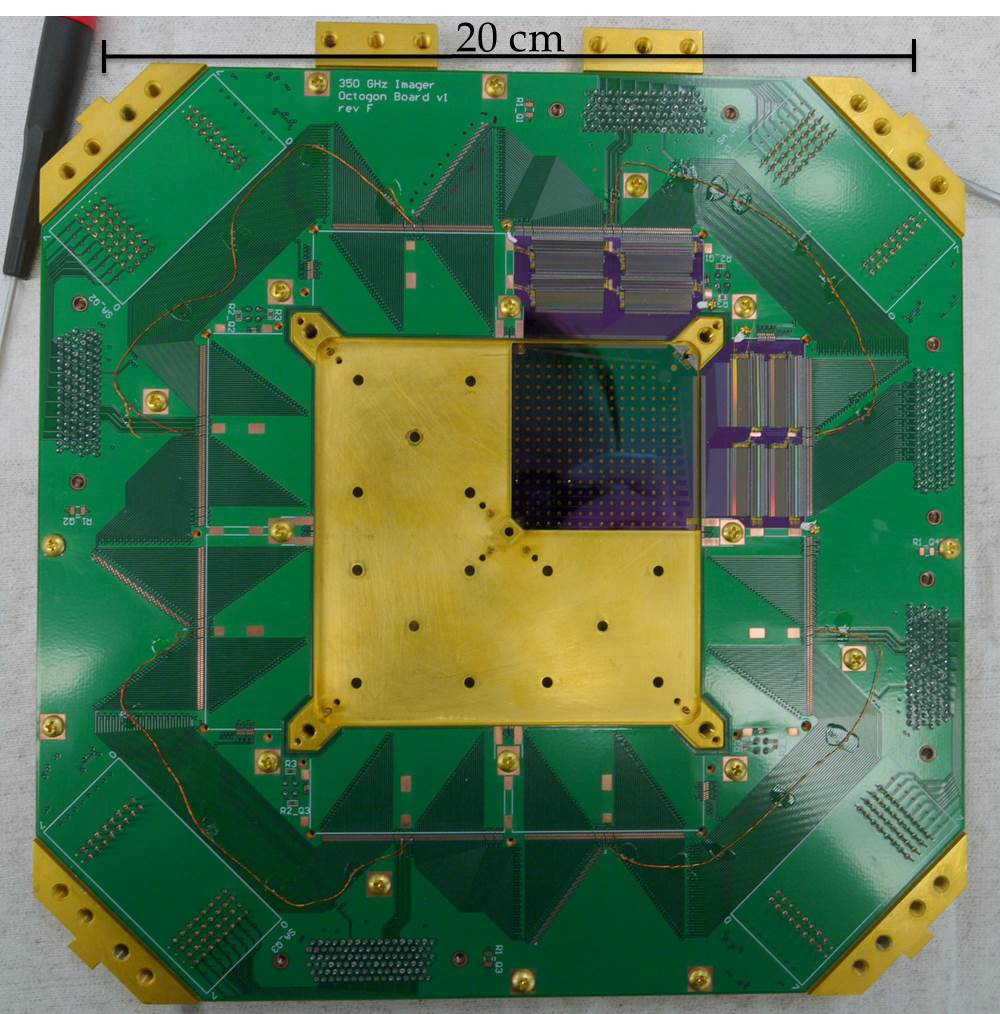
\includegraphics[width=6.0in]{../images/ch5-focal-plane-platter.jpg}};
    \begin{scope}[x={(image.south east)},y={(image.north west)}]
	    % \draw[help lines,xstep=.1,ystep=.1] (0,0) grid (1.0,1);
		% \foreach \x in {0,1,...,9} { \node [anchor=north] at (\x/10,0) {0.\x}; }
		% \foreach \y in {0,1,...,9} { \node [anchor=east] at (0,\y/10) {0.\y}; }
		
        \draw[black,ultra thick,rounded corners] (0.71,0.68) rectangle (0.50,0.83) node[below right] {\textbf{A}};
        \draw[black,ultra thick,rounded corners] (0.71,0.68) rectangle (0.85,0.48) node[above left] {\textbf{A}};
        \draw[black,ultra thick,rounded corners] (0.70,0.67) rectangle (0.50,0.44) node[above right] {\textbf{B}};

        \draw[black,ultra thick,<->] (.038,1.015) -- (0.965,1.015) node[midway,above] {\SI{9.5}{\in}}; % scale bar
    \end{scope}
\end{tikzpicture}

\end{document}
